\chapter{Introduction}

\begin{Abstract}
    \begin{changemargin}{2cm}{2cm}
    Dans ce premier chapitre, je ferai un survol historique de la physique
    unidimensionnelles pour motiver la recherche de ce mémoire. Si vous
    souhaitez avoir une introduction plus complète du domaine de recherche je
    conseille.... Ensuite, j'introduirai la problématique de ce mémoire pour
    ensuite enchaîner sur les différents morceaux du modèle de ce mémoire.
    Enfin, je ferai une première résolution du problème en utilisant la
    méthode de champ moyen pour donner une première intuition du modèle et
    pour justifer l'arrivé du prochain chapitre.
    \end{changemargin}
\end{Abstract}

\section{Histoire des matériaux unidimensionnels}
Commençons notre histoire en 1911 au Pays-Bas (Bien qu'on puisse toujours
commencer plus tôt), Avec Onnes qui mesure pour la première fois une
résistance électrique nulle dans le mercure (Hg). Ceci est la première
mesure d'une nouvelle phase.

\section{Contexte}

\section{Modèle Su-Schrieffer-Heeger (SSH)}
Le modèle Su-Schreiffer-Heigger apparaît pour la première fois en 1980
\cite{susoliton1980} pour tenter des résultats expérimentaux sur des
molécules organiques de polyacétylène \cite{goldberg-electron-1979}.
Alors, ils imaginent un modèle où l'on permet un déplacement entre-eux
des paires de carbone et hydrogène.
\begin{figure}[H]
    \centering
    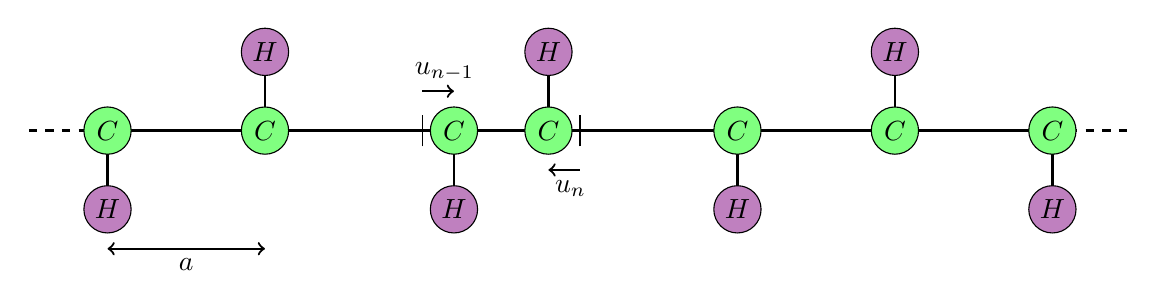
\begin{tikzpicture}
        \draw[thick] (-6,0) -- (6,0);
        \draw[thick, dashed] (-7,0) -- (-6,0);
        \draw[thick, dashed] (6,0) -- (7,0);
        \foreach \i in {-6,-4,2,4,6}{
        \draw[thick] (\i,0) -- (\i,{(-1)^(\i/2)});
        \draw[fill = green!50] (\i,0) circle [radius = 0.3cm] node{$C$};
        \draw[fill = violet!50] (\i,{(-1)^(\i/2)}) circle [radius = 0.3cm] node{$H$};
        }
        \draw[thick] (-1.6,0) -- (-1.6,-1);
        \draw[thick] (-0.4,0) -- (-0.4,1);
        \draw[fill = green!50] (-1.6,0) circle [radius = 0.3cm] node{$C$};
        \draw[fill = violet!50] (-1.6,{-1}) circle [radius = 0.3cm] node{$H$};
        \draw[fill = green!50] (-0.4,0) circle [radius = 0.3cm] node{$C$};
        \draw[fill = violet!50] (-0.4,{1}) circle [radius = 0.3cm] node{$H$};
        \draw[thick,<->](-6,-1.5) -- (-4,-1.5) node[pos = 0.5,below]{$a$};
        \draw (0,-0.2) --(0,0.2);
        \draw (-2,-0.2) --(-2,0.2);
        \draw[thick,->](0,-0.5) --(-0.4,-0.5) node[pos = 0.3,below]{$u_n$};
        \draw[thick,->](-2,0.5) --(-1.6,0.5) node[pos = 0.7,above]{$u_{n-1}$};
    \end{tikzpicture}
    \caption{Déformation du système représentant l'interaction des phonons
    du modèle SSH d'une molécule de polyacétilène. Le terme $u_n$ (un champ
    scalaire) représente la déformation de la paire d'atome par rapport à
    sa position d'équilibre}
\end{figure}
Ce modèle ne s'applique pas uniquement au polyacétylène, on peut
représenter ce modèle par n'importe quelle chaîne de molécules où les
molécules oscillent entre-elles. Dans ce cas, on représente une molécule
par un site du réseau et on modélise les phonons intermoléculaires, petit
par rapport à la distance entre les sites, par des oscillateurs harmoniques.
On peut représenter ce modèle avec le hamiltonien suivant où $t_{n,n+1}$ est
le terme de saut d'électrons et $u_n$ la déviation du site par rapport à sa
position d'équilibre.
\begin{align}
    H_{SSH} = -\sum_{\sigma,n} t_{n,n+1} \qty(c^\dagger_{n,\sigma}c_{n+1,\sigma}
    + c^\dagger_{n+1,\sigma}c_{n,\sigma} ) + \frac{1}{2}\sum_{n}
    \kappa (u_{n+1}-u_n)^2 + \frac{M}{2}\sum_n \dot{u}^2_n
\end{align}
Aussi, on pose la masse et la constant $\kappa$ comme uniforme (Symétrie de
translation).  Par la suite, le mouvement des sites imposent une variation
de la variable $t_{n,n+1}$, on pose alors une correction linéaire.
\begin{align}
    t_{n,n+1} \approx t_0 + t'(u_{n+1} - u_n)
\end{align}
Cette correction linéaire permet d'inclure une interaction entre les phonons
et les électrons. Donc,
\begin{align}
    H_{SSH} = -\sum_{\sigma,n} (t_0 + t'(u_{n+1} - u_n))
    \qty(c^\dagger_{n,\sigma}c_{n+1,\sigma} + c^\dagger_{n+1,\sigma}
    c_{n,\sigma} )+ \frac{1}{2}\sum_{n} \kappa (u_{n+1}-u_n)^2
    + \frac{M}{2}\sum_n \dot{u}^2_n
\end{align}
Maintenant, on fait une tranformation de Fourier et on utilise les définitions
suivante pour les opérateurs bosoniques qui permettrons de retrouver une
forme similaire à un oscillateur harmonique quantique.
\begin{align*}
    u_{n} =  \frac{1}{\sqrt{N}}\sum_{q}u_q e^{iqnd}\qquad\dot{u}_{n} =
    \frac{1}{\sqrt{N}}\sum_{q}p_q e^{iqnd}\qquad  c_{n,\sigma} =
    \frac{1}{\sqrt{V}}\sum_k c_{k,\sigma} e^{iknd} \\
\end{align*}
\begin{align*}
    u_q = \sqrt{\frac{1}{2M\omega(q)}}\qty(b_{q,b}+b^\dagger_{-q,b})\qquad
    p_q =\sqrt{\frac{M\omega(q)}{2}}\qty(b_{q,b}^\dagger-b_{-q,b}) \\
\end{align*}
On tombe sur l'hamiltonien suivant.
\begin{align}
    H_{SSH} = \underbrace{\sum_{k,\sigma}\epsilon(k)c_{k\sigma}^\dagger
    c_{k\sigma} + \sum_{\sigma,k,q}\frac{g(k,q)}{\sqrt{N}}
    c^\dagger_{k+q,\sigma}c_{k,\sigma}(b_q+b^\dagger_{-q})}_{H_e}
    + \underbrace{\sum_q\omega(q)\qty(b^\dagger_qb_q+\frac{1}{2})}_{H_{ph}^0},
\end{align}
où
\begin{align}
    \epsilon(k) &= -2t_0\cos(kd)\\
    g(k,q) &= \frac{-4it'\cos(\left[k+\frac{q}{2}\right]d)\sin
    \qty(\frac{qd}{2})}{\sqrt{2M\omega(q)}} \\
    \omega(q) &= -\sqrt{\frac{4\kappa}{M}} \sin\qty(\frac{qd}{2})
\end{align}
Avec $\epsilon(k)$ la relation de dispersion des électrons, $\omega(q)$
celle des phonons et la constante $g(k,q)$ représente la constante de
couplage électron-phonon.

\section{Modèle d'Holstein (ou Cristal Moléculaire)}
D'un autre côté, rien ne nous empêche d'imaginer des oscillations à même
le "site", c'est à dire l'existence de phonons intramoléculaires. Ce modèle
a été introduit par Holstein en 1959 lorsqu'il tentait d'étudier le
mouvement des polarons(une quasiparticule formé d'un électron localisé
avec une déformation du réseau)\cite{holstein-studies-1959}. Si on reprend
l'exemple du polyacétilène, on peut représenter ces phonons comme des
vibrations entre les atomes d'hydrogène et l'atome de carbone auquel ils
sont liés.
\begin{figure}[H]
    \centering
    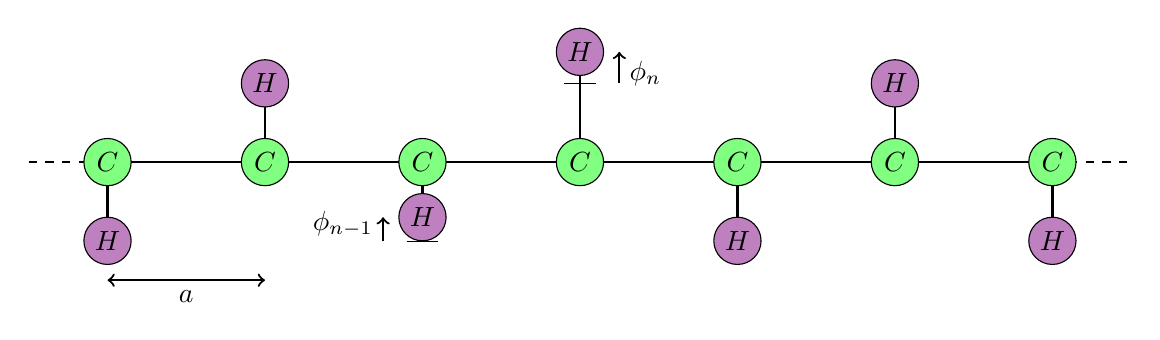
\begin{tikzpicture}
        \draw[thick] (-6,0) -- (6,0);
        \draw[thick, dashed] (-7,0) -- (-6,0);
        \draw[thick, dashed] (6,0) -- (7,0);
        \foreach \i in {-6,-4,2,4,6}{
        \draw[thick] (\i,0) -- (\i,{(-1)^(\i/2)});
        \draw[fill = green!50] (\i,0) circle [radius = 0.3cm] node{$C$};
        \draw[fill = violet!50] (\i,{(-1)^(\i/2)}) circle [radius = 0.3cm] node{$H$};
        }
        \draw[thick] (-2,0) -- (-2,-0.7);
        \draw[thick] (0,0) -- (0,1.4);
        \draw[fill = green!50] (-2,0) circle [radius = 0.3cm] node{$C$};
        \draw[fill = violet!50] (-2,-0.7) circle [radius = 0.3cm] node{$H$};
        \draw[fill = green!50] (-0,0) circle [radius = 0.3cm] node{$C$};
        \draw[fill = violet!50] (-0,1.4) circle [radius = 0.3cm] node{$H$};
        \draw[thick,<->](-6,-1.5) -- (-4,-1.5) node[pos = 0.5,below]{$a$};
        \draw (0.2,1) --(-0.2,1);
        \draw (-2.2,-1.01) --(-1.8,-1.01);
        \draw[thick,->](0.5,1) --(0.5,1.4) node[pos = 0.3,right]{$\phi_n$};
        \draw[thick,->](-2.5,-1)--(-2.5,-0.7) node[pos = 0.7,left]{$\phi_{n-1}$};
    \end{tikzpicture}
    \caption{Déformation du système représentant l'interaction des phonons
    du modèle d'Holstein. Le terme $\phi_n$ (un champ scalaire) représente
    la déformation de la paire d'atome par rapport à sa position
    d'équilibre}
\end{figure}
Contrairement au modèle précédent, ce type de phonon n'induit pas un déplacement
des sites du réseau mais plutôt une variatiton de la densité électronique "à
l'intérieur" des sites, d'où leur nom: intramoléculaire. On représente ce type
de phonon avec un opérateur $n_{i,\sigma} = c^\dagger_{i,\sigma}$
\begin{align}
    H_{CM} =-t\sum_{n,\sigma} c^\dagger_{n,\sigma}c_{n+1,\sigma}
    + c^\dagger_{n+1,\sigma}c_{n,\sigma}  + \lambda\sum_n\phi_n
    c^\dagger_{n,\sigma}c_{n,\sigma} + \frac{1}{2}\kappa^{M}\sum_n\phi_n^2
    + \sum_n\frac{M\dot{\phi}_n^2}{2}
\end{align}
On applique une transformation de Fourier sur les différents opérateurs
\begin{align*}
        \phi_{n} &=  \frac{1}{\sqrt{N}}\sum_{q}u_q e^{iqnd}\qquad\dot{\phi}_{n}
        =  \frac{1}{\sqrt{N}}\sum_{q}p_q e^{iqnd}\qquad  c_{n,\sigma}
        = \frac{1}{\sqrt{V}}\sum_k c_{k,\sigma} e^{iknd} \\
        x_q &= \sqrt{\frac{1}{2M\omega(q)}}\qty(b_{q,s}+b^\dagger_{-q,s})\qquad
        p_q =\sqrt{\frac{M\omega(q)}{2}}\qty(b_{q,s}^\dagger-b_{-q,s}) \\
\end{align*}
\section{Champ Moyen}
coucou, les copains
\begin{figure}[H]
    \centering
    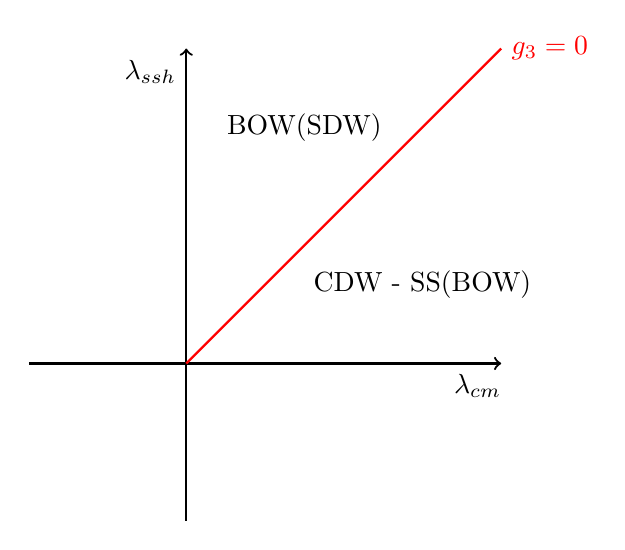
\begin{tikzpicture}
        \draw[->,thick] (-2,0)--(4,0) node[below, pos = 0.95]{$\lambda_{cm}$};
        \draw[->,thick] (0,-2)--(0,4)  node[left, pos = 0.95]{$\lambda_{ssh}$};
        \draw[thick,red] (0,0) -- (4,4) node[ right, pos = 1]{$g_3 = 0$};
        \node at (1.5,3) {BOW(SDW)};
        \node at (3,1) {CDW - SS(BOW)};
    \end{tikzpicture}
    \caption{Test de figure}
    \label{ttest}
\end{figure}
Ensuite, je fais un test de référence de figures \ref{ttest}.
